\chapter{Design Front-End}
\thispagestyle{stdPage}

%capo la mia conoscienza di latex si sta espandendo però probabilmente questo non compila comunque, halp me plz
% ho fatto del mio meglio per preparare un brodo degno di gordon ramsay

\section{Pagina Iniziale}

    \begin{figure}
        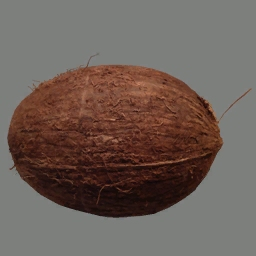
\includegraphics[width=\textwidth]{slides/placeholder.jpg} %PLACEHOLDER QUI CI VA LA PRIMA SLIDE DI LUCA
        \caption{Figura 1 PLACEHOLDER}
    \end{figure}

    La Figura 1 mostra un mockup della principale dell'applicazione, questa schermata sarà visibile a tutti gli utenti.

    \begin{itemize} %sono piuttosto sicuro che questa lista uscira tutta incasinata
        \item RF1: La homepage dell'applicazione mostra la mappa del Comune di Trento in primo piano, sono visibili anche i confini tra i singoli quartieri della città
        \item RF2: L'interfaccia contiene tre pulsanti, ognuno contenente una bandiera corrispondente a una delle lingue supportate dall'applicazione (italiano, inglese, tedesco). Cliccare sui pulsanti cambierà la lingua in cui è presentata l'interfaccia grafica 
        \item RF5: L'interfaccia presenta un pulsante, rappresentato da un'icona, che permette di iniziare il processo di autenticazione degli utenti. Questo permette agli utenti loggati di acceder al proprio account tramite SPID, CNS, CIE, CPS; come dettato dal requisito.
        \item RNF1: L'interfaccia usa un design semplice, che rende facile supportare l'uso dell'applicazione sui browswer Chrome, Firefox, Safari, Edge (come specificato dal requisito)
        \item RNF9: La grafica presentata all'utente utilizza un design chiaro, usando una top bar e icone per rendere la navigazione dell'interfaccia il più accessibile possibile
        \item RNF11: All'inizio, l'interfaccia sarà presentata in lingua italiana. Il design include modo di cambiare la lingua in inglese o tedesco
    \end{itemize}




\section{Selezione di un Quartiere}

    \begin{figure}
        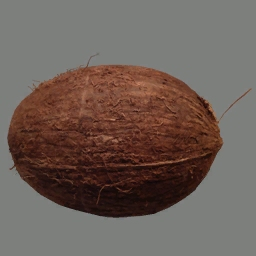
\includegraphics[width=\textwidth]{slides/placeholder.jpg} %PLACEHOLDER QUI CI VA LA SECONDA SLIDE DI LUCA
        \caption{Figura 2 PLACEHOLDER}
    \end{figure}    

    La Figura 2 mostra il mockup della schermata visibile dopo che l'utente ha cliccato su uno dei quartieri, l'immagine del quartiere è ingrandita per rendere chiaro che è stato selezionato

    \begin{itemize}
        \item RF3: Selezionare un qualunque dei quartieri di Trento sarà possibile con un click, una colta selezionato un quartiere, l'interfaccia dell'applicazione mostrerà i dati relativi a esso. La figura mostra solo i dati generali, visibili dagli utenti non loggati, una volta che un utente si sarà autenticato, verranno mostrati anche i dati più approfonditi
    \end{itemize}


%qui ci va la descrizione della terza immagine...